\PassOptionsToPackage{table}{xcolor} % load colortbl when xcolor is loaded - for coloring tables
\documentclass[10pt,twoside,sfsidenotes]{tufte-handout}

% --- Custom Preamble ---
\input{exam_preamble.tex} % loads packages, custom commands, etc.

% Metadata
\date{} % suppress date
\SetVariations{2}
\variant{1}

% Fancy headers/footers
\fancyhead[L]{MATH 2860 -- E04 --- \monthyear}
\fancyhead[R]{\textbf{Name (Last, First):} \blank[width=3in]{}}
% \fancyhead[R]{\textbf{Name} (Last, First): \blank[width=3in]{} \\
% \textbf{Circle your TA}: Trevor \quad Yuchen \quad Samantha }
\fancyfoot[R]{\thepage/\pageref{LastPage}}




%----------------------------------------------------------
% --- Document ---
\begin{document}
\setlength\abovedisplayskip{2pt}
\setlength\belowdisplayskip{2pt}
\setlength\abovedisplayshortskip{2pt}
\setlength\belowdisplayshortskip{2pt}

\vspace*{1in}


   {\large I will not violate the Clarkson University Code of Ethics or assist others in doing so, especially by presenting others' work as mine, or allow them to present my work as theirs. \textbf{I am better than that} and I take pride in, and responsibility for, my work. I understand that violations of the Code may result in loss of credit for the exam, the course, or even jeopardize my academic standing.

\vspace{.5in}

    \textbf{Signed:}
  }

  \vfill


\begin{center}\Large
  \begin{tabular}{c | c | c}
    Problem & Max & Scored \\ \hline
     & & \\ \hline
     & & \\ \hline
     & & \\ \hline
     & & \\ \hline
     & & \\ \hline
     & & \\ \hline
     & & \\ \hline
     & & \\ \hline
    Exam grade & & \\ \hline
  \end{tabular}
  \end{center}

  \vfill

  \begin{fullwidth}
{\large
  \begin{itemize}
    \item Start the exam only at the proctor's signal.
%    \item The last page in this booklet is the \textbf{formula sheet}. Feel free to carefully detach it from the booklet.
  \item Closed books and notes, no brought-in summary sheets, formula sheets, or any such accessories.
  \item No external paper allowed; if you need extra paper, please ask the proctor for it.
  \item Only basic sci. calculators allowed; no graphing, matrix, or CAS calculators.
  \item If needed, use both sides of each sheet for your answers. Clearly indicate where the answer is written, if it is not in the space provided for it.
  \end{itemize}
  }
\end{fullwidth}
\clearpage



% - Direction field, phase portrait
\begin{fullwidth}
    \begin{question}
        \begin{enumerate}[(i)]
            \item For what type of ODEs is the \textbf{phase portrait} a useful summary of the behavior of solutions? \solspace{0.5in}
            \item What is \vary{an equilibrium}{a semi-stable fixed point}? \solspace{0.5in}
            \item Calculate everything needed to sketch the phase portrait of the ODE:
                \vary{\[\frac{dy}{dx} = y(y-2)^{2} (y^{2} + 1) e^{-y}\]}{\[\frac{dy}{dx} = y^{2}(y-2) (y^{2} + 1) e^{-y}\]}
                and then sketch the phase portrait and \textbf{classify the type of fixed points}.
            \vfill
            \item \textbf{Sketch and label} the solution curves started at the following initial conditions as they extend into \(x\to\infty\):
                \begin{colenumerate}[4]
                    \item \(y(0) = 2\)
                    \item \(y(0) = 1\)
                    \item \(y(0) = -1\)
                    \item \(y(1) = 3\)
                \end{colenumerate}
        \end{enumerate}
        
        \begin{minipage}{0.3\linewidth}
            \centering
            Sketch of Phase Portrait

            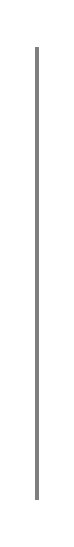
\begin{tikzpicture}[semitransparent]
                \path (0,0) node(x) {}
                (0,6) node(y) {};
                \draw[very thick] (x) -- (y);
            \end{tikzpicture}
        \end{minipage}
        \begin{minipage}{0.7\linewidth}
            \centering
            Sketch of Solution Curves

            \emptygrid[0.75]{10}{8}

            \textbf{\small Label the axes and the initial conditions.}
        \end{minipage}
    \end{question}
\end{fullwidth}



% - Linear 1st order ODE
\clearpage
\begin{question}
    \begin{enumerate}[(i)]
        \item Show that one of the following ODEs is exact and the other is linear. \\ Show your work for \textbf{both} ODEs.
            \begin{fullwidth}
                \begin{colenumerate}
                \item \(\displaystyle \vary{\frac{1}{t^2} \frac{dx}{dt} + x - e^{t^{3}} = 0}{[5x-2t^{2}] \frac{dx}{dt} = 4t\cdot x - t},\)
                \item \(\displaystyle \vary{[5x-2t] \frac{dx}{dt} - 2x = 0}{\frac{1}{t} \frac{dx}{dt} = -t \cdot x + t\cdot e^{t^{3}}}.\)
                \end{colenumerate}
            \end{fullwidth}
            \vfill
        \item 
            \begin{fullwidth}
                Solve \textbf{one} of the two ODEs given above (whichever you personally prefer). \textbf{Show your work.}
            \end{fullwidth}
            \vfill
    \end{enumerate}
\end{question}


% - Homogeneous ODE; damping (sketch)
\clearpage
\begin{question}
    The following ODE has a positive damping parameter \(c \geq 0\) in it:\vary{\[y''(x) + c y'(x) + 4 y(x) = 16\]}{\[y''(x) + c y'(x) + 9 y(x) = 18\]}

    \begin{enumerate}[(i)]
        \item Calculate the particular solution for \vary{\(c = 5\), \(y(0) = 1\), \(y'(0) = 1\).}{\(c = 10\), \(y(0) = 0\), \(y'(0) = -2\).}
        \item Sketch the solution from (i) into the grid, according to the guidelines.
            \begin{marginfigure}
                \centering
                Space for the solution sketch.
                \emptygrid[0.75]{6}{6}
                \textbf{Guidelines.} Accurately represent:\\
                \begin{inparaitem}
                    \item initial value
                    \item sign of the initial slope,
                    \item presence/absence of oscillations,
                    \item limit as \(x \to \infty\).
                \end{inparaitem}
                \textbf{Label the axes.}
            \end{marginfigure}
        \item Use the characteristic equation and its roots to determine the \textbf{range of positive values} of \(c\) for which the solutions \textbf{do not} have any oscillations.
    \end{enumerate}
    \begin{center}
        \textsc{\small Use empty space below as needed, but label important parts of your calculations.}
    \end{center}
\end{question}



% - Inhomogeneous ODE; resonance
\clearpage
\begin{question}
    The sketch shows a mechanical system. \(x(t)\) is the displacement of the body at time \(t\), \(f(t)\) is the force that is applied at the center of the mass of the body.
    \begin{marginfigure}\centering
        \includegraphics[width=0.9\linewidth]{Exam_figs/cart}

        \vspace{2em}

        \textsc{Use empty space below as needed, but label important parts of your calculations.}
    \end{marginfigure}

    \begin{enumerate}[(i)]
        \item \textbf{Use a free-body diagram and Newton's laws of motion} to derive the ODE for the position of the body \(x(t)\). \textbf{Make sure to show your work.}
        \item Explain in your words, what is \textbf{resonance}?
        \item If the external force is \(f(t) = \cos( \vary{2}{3} t)\), what value of the spring constant \(k\) is needed for the body of mass \(m = \vary{2}{4}\) to be in resonance with the input?
    \end{enumerate}
\end{question}



% inhomogeneous ODE
\clearpage
\begin{question} \marginnote{Table of Laplace transform is on the last page if you need it.}
    Use \textbf{any technique} to calculate the \textbf{general} solution of: \[
        \ddot x(t) + 2 x(t) + 10 x(t) = t + e^{-2t}
    \]
\end{question}

%
\clearpage
\begin{question}
    Use Laplace transform to calculate the solution to the ODE below. \marginnote{Note: \(\delta(t)\) stands for the Dirac \(\delta\)-impulse. Table of Laplace transform is on the last page.}:
    \[
        y''(t) + 4y'(t) + 3y(t) = \delta(t-1), \quad y'(0) = 0,\ y(0) = 3.
    \]
\end{question}


\clearpage
\begin{question} % Shift in time domain, shift in s-domain
    \begin{enumerate}[(i)]
        \item Compute and \textbf{sketch}:
            \(\displaystyle
            g(t) = \laplace^{-1}\braced*{\frac{1}{s} + \frac{2}{s^{2}}e^{-s} - \frac{2}{s^{2}}e^{-2s}}
            \)
        \vfill

        \item Compute:
            \( \displaystyle
            F(s) = \laplace\braced*{(t^{2}-t)\hstep(t-1)}
            \)

        \vfill
  \end{enumerate}
\end{question}



% - Phase portrait ODE system (extra credit: use exact equation to find implicit formula for solution curves)
\clearpage
\begin{question}
    The ODE system is given by the following equations:
    \[
        \begin{aligned}
        \dot x(t) &= 2x(t) - 5y(t) \\
        \dot y(t) &= 4x(t) -2y(t)
        \end{aligned}
    \]

    \begin{enumerate}[(i)]
        \item Calculate everything needed to sketch a phase portrait.


        \item
            \begin{marginfigure}\centering
                Space for phase portrait sketch.
                \emptygrid[0.75]{6}{6}
                \textbf{Guidelines.} Accurately represent:
                \begin{inparaitem}
                    \item location of the fixed point,
                    \item presence/absence of oscillations,
                    \item growth/decay (or neither) of solutions,
                    \item characteristic directions (if applicable).
                \end{inparaitem}
                \textbf{Label the axes.}
            \end{marginfigure}
        Based on your calculations in (i) sketch the phase portrait.

        \item (Extra credit) Calculate the implicit formula \(E(x,y) =\text{const.}\)
        for the solution curves using the procedure analogous to the one in Project 3.
    \end{enumerate}

    \begin{center}
        \textsc{\small Use empty space below as needed, but label important parts of your calculations.}
    \end{center}
\end{question}


% - 3x3 eigenvector calculation, eigenvector candidate, general solution
\clearpage
\begin{question}
    Given is the matrix ODE:  
    \begin{marginfigure}
        \centering
        \textsc{Use empty space below as needed, but label important parts of your calculations.}
    \end{marginfigure}
    
    \[\begin{bmatrix}
        \dot x(t) \\\dot y(t) \\\dot z(t)
    \end{bmatrix}
    =
    \underbrace{\begin{bmatrix}
       -1 & 0 &  0  \\
        1 & 6 & -10 \\
        0 & 4 & -6
    \end{bmatrix}}_{\mm{M}}
        \begin{bmatrix}
        \dot x(t) \\\dot y(t) \\\dot z(t)
    \end{bmatrix}
    \]

    \begin{fullwidth}
        \begin{enumerate}[(i)]
            \item Verify that the eigenvalues of matrix \(\mm{M}\)  are \(\lambda_{1} = -1, \lambda_{2,3} = \pm 2i\).
            \item Verify that the vector \(\vv{v} =
                \begin{smallbmatrix}
                    5 \\ 5 \\ 4
                \end{smallbmatrix}\cdot\alpha
                \) is an eigenvector of the matrix \(\mm{M}\).
            \item Calculate the remaining two eigenvectors.
            \item Write out a general solution of the matrix ODE. (For full credit, use real-valued form of the characteristic solutions associated to complex eigenvalues).
        \end{enumerate}
    \end{fullwidth}
\end{question}

\clearpage
\begin{minipage}{0.5\linewidth}
%
      Laplace integral:

      $\laplace\braced*{f(t)} = \int_0^{\infty} e^{-st}
f(t)dt $

Properties, given that

$\laplace\braced*{f(t)} = F(s)$, $\laplace\braced*{g(t)} = G(s)$:

\begin{itemize}
\item Linearity: \\$
  \begin{aligned}
\laplace&\braced*{c_1f(t)+c_2g(t)} \\&= c_1F(s) + c_2G(s)
\end{aligned}
$
\item \(s\)-shift:  \\ $\laplace\braced*{e^{at}f(t)} = F(s-a)$
\item \(t\)-shift: \\ $\laplace\braced*{\hstep(t-a)f(t-a)} = e^{-sa}F(s)$

\item Derivative in \(t\): If $\laplace\braced*{y(t)} = Y(s)$, then
  \begin{align*}
    \laplace\braced*{y'(t)} &= sY(s)-y(0), \\
    \laplace\braced*{y''(t)} &= s^2Y(s) - sy(0) - y'(0)
  \end{align*}

\end{itemize}

  \begin{center}
\rowcolors{1}{white}{gray!15}
\renewcommand{\arraystretch}{2}
\begin{tabular}{ |>{\centering\arraybackslash}m{0.5in}|>{\centering\arraybackslash}m{0.5in}|}
  $f(t)$ & $F(s) = \laplace\braced*{f(t)}$\\\hline
$\delta(t)$ & $1$ \\
  $1$ & $\frac{1}{s}$ \\
  $\hstep(t)$ & $\frac{1}{s}$ \\
$t^n$ & $\frac{n!}{s^{n+1}}$ \\
$e^{at}$ & $\frac{1}{s-a}$ \\
$\sin(\omega t)$ & $\frac{\omega}{s^2+\omega^2}$ \\
$\cos(\omega t)$ & $\frac{s}{s^2+\omega^2}$ \\
$e^{at}\sin(\omega t)$ & $\frac{\omega}{(s-a)^2+\omega^2}$ \\
$e^{at}\cos(\omega t)$ & $\frac{s-a}{(s-a)^2+\omega^2}$ \\
$\cosh(at)$ & $\frac{s}{s^2-a^2}$ \\
$\sinh(at)$ & $\frac{a}{s^2-a^2}$ \\
\end{tabular}
\end{center}

\end{minipage}
\begin{minipage}{0.5\linewidth}

      Laplace integral:

      $\laplace\braced*{f(t)} = \int_0^{\infty} e^{-st}
f(t)dt $

Properties, given that

$\laplace\braced*{f(t)} = F(s)$, $\laplace\braced*{g(t)} = G(s)$:

\begin{itemize}
\item Linearity: \\$
  \begin{aligned}
\laplace&\braced*{c_1f(t)+c_2g(t)} \\&= c_1F(s) + c_2G(s)
\end{aligned}
$
\item \(s\)-shift:  \\ $\laplace\braced*{e^{at}f(t)} = F(s-a)$
\item \(t\)-shift: \\ $\laplace\braced*{\hstep(t-a)f(t-a)} = e^{-sa}F(s)$

\item Derivative in \(t\): If $\laplace\braced*{y(t)} = Y(s)$, then
  \begin{align*}
    \laplace\braced*{y'(t)} &= sY(s)-y(0), \\
    \laplace\braced*{y''(t)} &= s^2Y(s) - sy(0) - y'(0)
  \end{align*}

\end{itemize}

  \begin{center}
\rowcolors{1}{white}{gray!15}
\renewcommand{\arraystretch}{2}
\begin{tabular}{ |>{\centering\arraybackslash}m{0.5in}|>{\centering\arraybackslash}m{0.5in}|}
  $f(t)$ & $F(s) = \laplace\braced*{f(t)}$\\\hline
$\delta(t)$ & $1$ \\
  $1$ & $\frac{1}{s}$ \\
  $\hstep(t)$ & $\frac{1}{s}$ \\
$t^n$ & $\frac{n!}{s^{n+1}}$ \\
$e^{at}$ & $\frac{1}{s-a}$ \\
$\sin(\omega t)$ & $\frac{\omega}{s^2+\omega^2}$ \\
$\cos(\omega t)$ & $\frac{s}{s^2+\omega^2}$ \\
$e^{at}\sin(\omega t)$ & $\frac{\omega}{(s-a)^2+\omega^2}$ \\
$e^{at}\cos(\omega t)$ & $\frac{s-a}{(s-a)^2+\omega^2}$ \\
$\cosh(at)$ & $\frac{s}{s^2-a^2}$ \\
$\sinh(at)$ & $\frac{a}{s^2-a^2}$ \\
\end{tabular}
\end{center}

\end{minipage}

\end{document}